\subsection{Schema information}
To initialize the history database the administrator runs the script \textit{history.py}.
It starts by creating the \textit{schema information tables} which Marty uses to store information about the schema of the master database:

\begin{description}
  \item[marty\_schemas]
    Contains the name and ID of all schemas in the slave database.
  \item[marty\_tables]
    Contains the name and ID of the tables in the slave database and a reference to the schema they are in.
    It also stores the \textit{internal name} which is used for the data table in the history and clone databases.
  \item[marty\_columns]
    Contains the name, number, type and length of each column in the tables.
    It also stores an internal name for the column that is used in the data tables in the history and clone databases.
\end{description}

Tables \ref{tbl:marty-schemas} to \ref{tbl:marty-columns} show information about the columns of these tables.
Note that each table contains a column called \textit{\_ctid}, see Chapter \ref{ch:implementation-history-ctid} for more information about the value in this column.
The tables also have two columns called \textit{start} and \textit{stop}.
These columns define which \textit{history version} each row is part of, see chapter \ref{ch:implementation-history-versions} for further information.
Figure \ref{fig:schema-information-example} shows an example of the contents of the schema information tables.

\begin{table}[h]
  \centering
  \textbf{marty\_schemas}
  \begin{tabularx}{\textwidth}{llX}
    \textit{Column} & \textit{Type} & \textit{Description} \\
    \midrule
    \_ctid & tid & A reference to the pg\_namespace table in the slave database \\
    oid & oid & The ID of the schema in the slave database \\
    name & name & The name of the schema \\
    start & integer & First version where this schema is present in the database \\
    stop & integer & First version where this schema stops being present in the database \\
  \end{tabularx}
  \caption{The columns of the marty\_schemas table}
  \label{tbl:marty-schemas}
\end{table}

\begin{table}[h]
  \centering
  \textbf{marty\_tables}
  \begin{tabularx}{\textwidth}{llX}
    \textit{Column} & \textit{Type} & \textit{Description} \\
    \midrule
    \_ctid & tid & A reference to the pg\_class table in the slave database \\
    oid & oid & The ID of the table in the slave database \\
    name & name & The name of the table \\
    schema\_oid & oid & A reference to the schema that this table belongs to \\
    internal\_name & name & The name of the data table, see Chapter \ref{ch:implementation-history-data} \\
    start & integer & First version where this table is present in the database \\
    stop & integer & First version where this table stops being present in the database \\
  \end{tabularx}
  \caption{The columns of the marty\_tables table}
  \label{tbl:marty-tables}
\end{table}

\begin{table}[h]
  \centering
  \textbf{marty\_columns}
  \begin{tabularx}{\textwidth}{llX}
    \textit{Column} & \textit{Type} & \textit{Description} \\
    \midrule
    \_ctid & tid & A reference to the pg\_attribute table in the slave database \\
    table\_oid & oid & A reference to the table this column is in \\
    name & name & The name of the column \\
    number & int2 & The index of this column in the table (is it the first, second, third etc.) \\
    type & name & The type of the column (int, text, boolean etc.) \\
    length & int4 & The length of the column. Some data types require the user to specify a length, such as character columns, e.g. char(26). Columns without length usually have the value -1 \\
    internal\_name & name & The name of this column in the data table, see Chapter \ref{ch:implementation-history-data} \\
    start & integer & First version where this column is part of the table \\
    stop & integer & First version where this column stops being part of the table \\
  \end{tabularx}
  \caption{The columns of the marty\_tables table}
  \label{tbl:marty-columns}
\end{table}

Postgres uses \textit{system catalogs} to store information about the schema of its databases.
They are used internally, e.g. when Postgres reads from or writes to tables.
Information such as which file in the database cluster represents which table and the column names and types of each table are stored in the system catalogs.
They are ordinary tables which are stored in a schema called \textit{pg\_catalogs} and can by queried by a user just as any other table.

Marty reads information from four system catalogs in the slave database:

\begin{description}
  \item[pg\_namespace]
    Contains information about the schemas in the slave database.
    Information from this catalog is saved in \textit{marty\_schemas} in the history database.
  \item[pg\_class]
    Contains information about the tables in the slave database.
    Information from this catalog is saved in \textit{marty\_tables} in the history database.
  \item[pg\_attribute]
    Contains information about the columns of the tables in the slave database.
    Information from this catalog is saved in \textit{marty\_columns} in the history database.
  \item[pg\_type]
    Contains additional information about the columns.
    Marty reads the name of the column type from this table (integer, text etc.) and stores it in \textit{marty\_columns} along with the other column related information.
\end{description}

The history.py script creates the schema information tables and then it populates them with information about the schema of the slave database.
This is of course also the schema of the master database so the history database really contains information about the master.

Marty inspects the schema of the slave database before any WAL records have been applied to it.
It writes the schema information to the history database, which creates the first history version, see Chapter \ref{ch:implementation-history-versions} for more about history versions.
Marty then starts the WAL replay in the slave database and reads the replay log.

When a new schema is created the WAL contains an \textit{insert} heap record for the pg\_namespace table.
Marty sees this in the replay log and queries the slave about this new schema.
It then creates a new history version that includes it.
The same happens when a new table is created or a new column is added to a table; a new history version is created that includes the new table or column.

If a schema, table, or a column is altered, e.g. when they are renamed, the WAL has an \textit{update} heap record.
Similarly when a schema, table or column is dropped the WAL has a \textit{delete} heap record.
Marty sees this in the replay log and creates new history versions with the altered database schema.

\begin{figure}[h!]
  \centering
    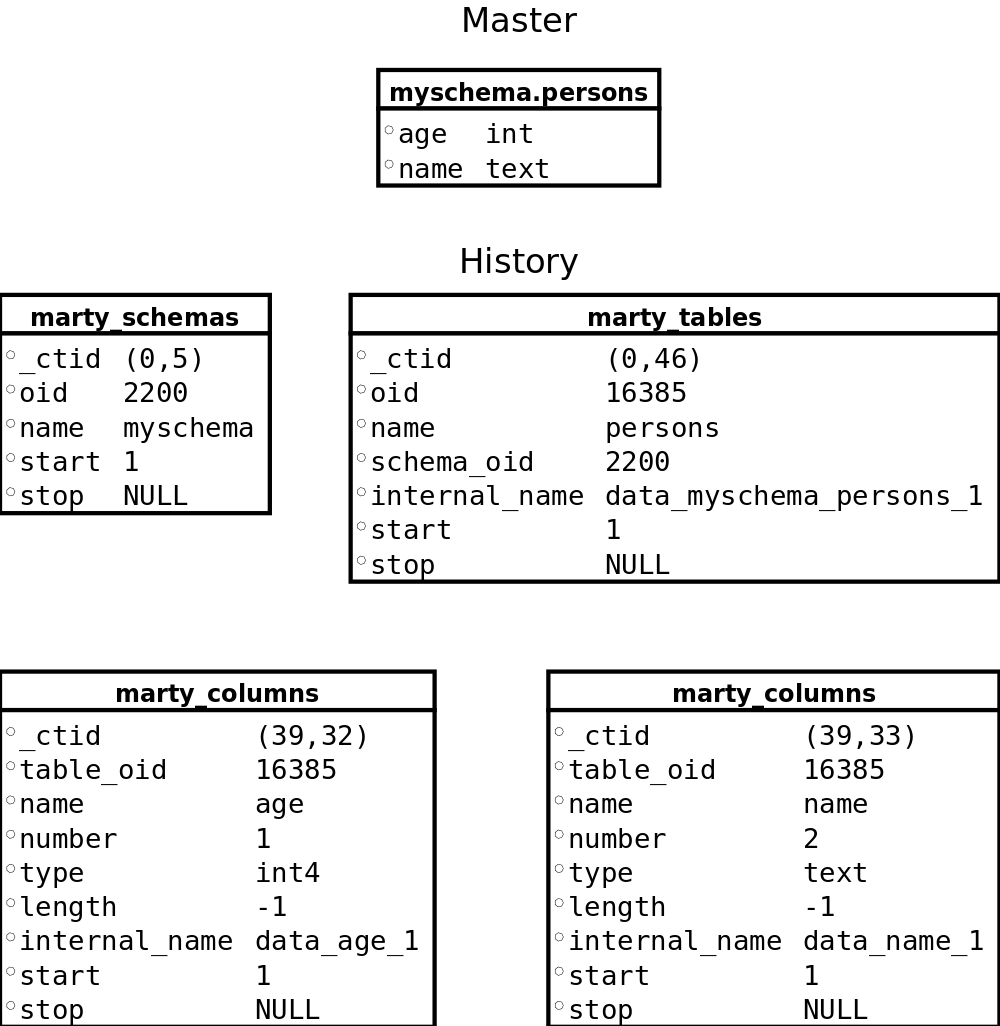
\includegraphics[width=0.75\textwidth]{schema-information-example}
  \caption{Example of the contents of the schema information tables}
  \label{fig:schema-information-example}
\end{figure}

See Figure \ref{fig:schema-information-example} for an example of the contents of the schema information tables.

In the example the master database has a schema called \textit{myschema}.
Its object identifier (oid) is 2200.
The \textit{pg\_namespace} system catalog in the slave database stores information about this schema in a row with the ctid value of (0,5).
This is reflected in the \textit{marty\_schemas} table in the history database.

The master contains one table, \textit{persons}, which belongs to myschema.
Information about this table is stored in \textit{marty\_tables}.
Its oid is 16385 and the slave stores information about this table in a row with ctid value of (0,46) in the \textit{pg\_class} system catalog.
Its internal name is \textit{data\_myschema\_persons\_1}, see Chapter \ref{ch:implementation-history-data} for information about internal names of tables and columns.

The persons table has two columns, \textit{age} of type \textit{integer} or \textit{int4}, and \textit{name} of type \textit{text}.
The slave stores information about these columns in the \textit{pg\_attribute} system catalog in rows with ctid values of (39,32) and (39,33).
The age column is the first column in the table, the name column is the second one.
This is reflected in the \textit{number} value in \textit{marty\_columns}.
Columns of type integer and text do not use the length attribute, so Postgres puts -1 there.
The internal names of the columns are \textit{data\_age\_1} and \textit{data\_name\_1}.

The schema, table and columns are all part of the first history version.
This is reflected in the columns \textit{start} in the schema information tables.
They have not yet been altered or dropped and are thus part of every history version after the first one, which is reflected with the NULL value in the \textit{stop} column.
See Chapter \ref{ch:implementation-history-versions} for information about history versions.